%----------------------------------------------------------------------------------
% Exemplo do uso da classe tcc.cls. Veja o arquivo .cls
% para mais detalhes e instruções.
%----------------------------------------------------------------------------------

% Seleção de idioma da monografia. Por enquanto as únicas opções
% suportadas são 'portuguese' e 'english'
% Para impressão em frente e verso, use a opção 'twoside'. Da
% mesma forma, use 'oneside' para impressão em um lado apenas.
\documentclass[portuguese,oneside]{tcc}

% \usepackage{xcolor}
%----------------------------------------------------------------
% Coloque seus pacotes abaixo.
%
% Obs.: muitos pacotes de uso comum do LaTeX, como amsmath,
% geometry e url já são automaticamente incluídos pela classe
% (veja o arquivo .cls). Isso torna obrigatória a presença destes
% no sistema para o uso desta classe, mas ao mesmo tempo o uso se
% torna mais simples.  Recomendo a instalação da versão mais
% recente da distribuição TeXLive (para Windows e UNIXes):
% www.tug.org/texlive/
%
% Pacotes e opções já incluídas automaticamente:
%
% \RequirePackage[T1]{fontenc}[2005/09/27]
% \RequirePackage[utf8x]{inputenc}[2008/03/30]
% \RequirePackage[english,brazil]{babel}[2008/07/06]
% \RequirePackage[a4paper]{geometry}[2010/09/12]
% \RequirePackage{textcomp}[2005/09/27]
% \RequirePackage{lmodern}[2009/10/30]
% \RequirePackage{indentfirst}[1995/11/23]
% \RequirePackage{setspace}[2000/12/01]
% \RequirePackage{textcase}[2004/10/07]
% \RequirePackage{float}[2001/11/08]
% \RequirePackage{amsmath}[2000/07/18]
% \RequirePackage{amssymb}[2009/06/22]
% \RequirePackage{amsfonts}[2009/06/22]
% \RequirePackage{url}
% \RequirePackage[table]{xcolor}[2007/01/21]
%----------------------------------------------------------------
% Para inserção de figuras.
\usepackage{graphicx}
% Utilize a opção 'pdftex' se você estiver usando o pdflatex (que
% permite figuras em formatos como .jpg ou .png)
%\usepackage[pdftex]{graphicx}

% Para tabelas com elementos ocupando mais de uma linha
\usepackage{multirow}
% Para frações na mesma linha (ex. ⅓).
\usepackage{nicefrac}
% Para inserir figuras lado a lado.
% \usepackage{subfigure}
% Para formatar algoritmos.
% A opção [algo2e] é necessária para evitar conflitos
% com as definições da classe.
%\usepackage[ruled, algo2e, linesnumbered]{algorithm2e}
%\usepackage{algorithmic}
% Um float do tipo algoritmo. No momento
% este pacote é incompatível com a classe.
%\usepackage{algorithm}
\usepackage[disable]{todonotes}
\usepackage{pgfgantt}
\usepackage{algpseudocode}
\usepackage{alltt}
%\usepackage{algorithm}
\newcommand\msr[2][noinline]{\todo[author=Matheus,color=blue!50,#1]{#2}}
\newcommand\frm[2][noinline]{\todo[size=\tiny,author=Felipe,color=red!75,#1]{#2}}



\usepackage{listings}
\usepackage{listingsutf8}

\lstset{literate=
	{ã}{{\~a}}1 {ẽ}{{\~e}}1 {ĩ}{{\~i}}1 {õ}{{\~o}}1 {ũ}{{\~u}}1
	{Ã}{{\~A}}1 {Ẽ}{{\~E}}1 {Ĩ}{{\~I}}1 {Õ}{{\~O}}1 {Ũ}{{\~U}}1	
	{á}{{\'a}}1 {é}{{\'e}}1 {í}{{\'i}}1 {ó}{{\'o}}1 {ú}{{\'u}}1
	{Á}{{\'A}}1 {É}{{\'E}}1 {Í}{{\'I}}1 {Ó}{{\'O}}1 {Ú}{{\'U}}1
	{à}{{\`a}}1 {è}{{\`e}}1 {ì}{{\`i}}1 {ò}{{\`o}}1 {ù}{{\`u}}1
	{À}{{\`A}}1 {È}{{\'E}}1 {Ì}{{\`I}}1 {Ò}{{\`O}}1 {Ù}{{\`U}}1
	{ä}{{\"a}}1 {ë}{{\"e}}1 {ï}{{\"i}}1 {ö}{{\"o}}1 {ü}{{\"u}}1
	{Ä}{{\"A}}1 {Ë}{{\"E}}1 {Ï}{{\"I}}1 {Ö}{{\"O}}1 {Ü}{{\"U}}1
	{â}{{\^a}}1 {ê}{{\^e}}1 {î}{{\^i}}1 {ô}{{\^o}}1 {û}{{\^u}}1
	{Â}{{\^A}}1 {Ê}{{\^E}}1 {Î}{{\^I}}1 {Ô}{{\^O}}1 {Û}{{\^U}}1
	{œ}{{\oe}}1 {Œ}{{\OE}}1 {æ}{{\ae}}1 {Æ}{{\AE}}1 {ß}{{\ss}}1
	{ű}{{\H{u}}}1 {Ű}{{\H{U}}}1 {ő}{{\H{o}}}1 {Ő}{{\H{O}}}1
	{ç}{{\c c}}1 {Ç}{{\c C}}1 {ø}{{\o}}1 {å}{{\r a}}1 {Å}{{\r A}}1
	{€}{{\EUR}}1 {£}{{\pounds}}1
}

\lstdefinestyle{codeStyle}{
	commentstyle=\color{black},
	basicstyle=\ttfamily\footnotesize,
	breakatwhitespace=false,         
	breaklines=true,                 
	captionpos=b,                    
	keepspaces=true,                 
	numbers=left,                    
	numbersep=5pt,                  
	showspaces=false,                
	showstringspaces=false,
	showtabs=false,                  
	tabsize=2
}


%----------------------------------------------------------------
% Autor (OBRIGATÓRIO)
%----------------------------------------------------------------
\author{Matheus de Souza Redecker}

%----------------------------------------------------------------
% Título (OBRIGATÓRIO). Devem ser passados DOIS parâmetros,
% o título em português E o inglês, não importando o idioma
% escolhido. Os títulos são utilizados para a montagem da capa,
% resumo e abstract mais tarde.
%----------------------------------------------------------------
\title{Adversarial Hierarchical-Task Network para Jogos em Tempo Real}
      {Adversarial Hierarchical-Task Network for Real-Time Games}

%----------------------------------------------------------------
% Opções para o tipo de trabalho (OBRIGATÓRIO)
%----------------------------------------------------------------
%\tipotrabalho{\ptci}         % Proposta de Trabalho de Conclusão
%\tipotrabalho{\tci}         % Trabalho de Conclusão I
\tipotrabalho{\tcii}        % Trabalho de Conclusão II

%----------------------------------------------------------------
% Seleção do curso ("este trabalho é um requisito parcial para
% obtenção do grau de (mestre ou doutor) em Ciência da Computação").
%----------------------------------------------------------------
\curso{\cc} % Ciência da Computação
%\curso{\si} % Sistemas de Informação
%\curso{\es} % Engenharia de Software

%----------------------------------------------------------------
% Orientador (e Co-orientador, caso haja um). É OBRIGATÓRIO
% informar pelo menos o orientador.
%----------------------------------------------------------------
\orientador{Felipe Rech Meneguzzi}
%\coorientador{Ciclano de Farias}

%----------------------------------------------------------------
% A capa é inserida automaticamente. Por isso não é necessário
% chamar \maketitle
%----------------------------------------------------------------
\begin{document}
%----------------------------------------------------------------
% Depois da capa vem a dedicatória e a epígrafe.
%----------------------------------------------------------------
%\dedicatoria{Dedico este trabalho a meus pais.}

%\epigrafe{The art of simplicity is a puzzle of complexity.}
         %{Douglas Horton}

%----------------------------------------------------------------
% Também dá para fazer as duas na mesma página:
%----------------------------------------------------------------
%\dedigrafe{Dedico este trabalho a meus pais.}
%          {The art of simplicity is a puzzle of complexity.}
%          {Douglas Horton}

%----------------------------------------------------------------
% A seguir, a página de agradecimentos (OPCIONAL):
%----------------------------------------------------------------
\begin{agradecimentos}
Inicialmente agradeço ao meu orientador prof. Felipe Rech Meneguzzi pela oportunidade de realizar este trabalho, sob sua orientação. 
Agradeço aos meus pais, Ana e Hélio, pelo suporte oferecido ao longo da vida acadêmica. E como não poderia deixar de mencionar, minha companheira, Carolina, pelo apoio, carinho, e pela compreensão em relação ao meu esforço na elaboração deste trabalho.
\end{agradecimentos}

%----------------------------------------------------------------
% Resumo, com as palavras-chave passadas por parâmetro
% (OBRIGATÓRIO, ao menos para teses e dissertações)
%----------------------------------------------------------------
\begin{resumo}{planejamento automatizado, planejamento hierarquico, busca adversária}
Jogos de estratégia em tempo real são difíceis do ponto de vista da Inteligência Artificial (IA) devido ao grande espaço de estados e a limitação do tempo para tomar uma ação. 
Uma abordagem recentemente proposta é combinar busca adversária com técnicas de HTN, o algoritmo é chamado de \textit{Adversarial Hierarchical-Task Network}.
Propomos a utilização deste algoritmo em um jogo de estratégia em tempo real.
\end{resumo}

%----------------------------------------------------------------
% Abstract, com as palavras-chave passadas por parâmetro
% (OBRIGATÓRIO, ao menos para teses e dissertações)
%----------------------------------------------------------------
\begin{abstract}{automated planning, hierarchical planning, adversarial search}
Real-time strategy games are hard from an Artificial Intelligence (AI) point of view due to the large state-spaces and the short time to compute each player's action. 
A recently proposed approach is to combine adversarial search techniques with HTN techniques, in an algorithm called Adversarial Hierarchical-Task Network. 
We propose the utilization of this algorithm in one real-time strategy game.
\end{abstract}

%----------------------------------------------------------------
% Listas e sumário, nessa ordem. Somente o sumário é obrigatório,
% portanto, comente as outras listas, caso sejam desnecessárias.
%----------------------------------------------------------------
%\frm[inline]{Ele não compila direito comigo, algo a ver com a lista de algoritmos}
%\msr[inline]{ele está com um problema na biblioteca dos algoritmos, estou tentando resolver}

\listoffigures       % Lista de figuras      (OPCIONAL)
%\listoftables        % Lista de tabelas      (OPCIONAL)
\listofalgorithms    % Lista de algoritmos   (OPCIONAL)
\listofacronyms      % Lista de siglas       (OPCIONAL)
%\listofabbreviations % Lista de abreviaturas (OPCIONAL)
%\listofsymbols       % Lista de símbolos     (OPCIONAL)
\tableofcontents     % Sumário               (OBRIGATÓRIO)

%----------------------------------------------------------------
% Aqui começa o desenvolvimento do trabalho. Para uma melhor
% organização do documento, separe-o em arquivos,
% um para cada capítulo. Para isso, utilize o comando \include,
% como mostrado abaixo.0
%----------------------------------------------------------------

\sigla{IA}{Artificial Intelligence}
\sigla{HTN}{Hierarchical Task Network}
\sigla{AHTN}{Adversarial Hierarchical Task Network} 
\sigla{RTS}{Real-time Strategy}
\sigla{TFD}{Total-order Forward Decomposition}

%!TEX root = volumeFinal.tex 
\chapter{\label{chap:intro}Introdução}

A Inteligência Artificial (IA) possui aplicação em jogos, fazendo com que os computadores sejam capazes de jogar jogos como xadrez e jogo da velha sem intervenção humana. 
Os jogos de computador muitas vezes não utilizam algoritmos de IA para simular o comportamento dos jogadores, utilizando ao invés disso, técnicas que passam a ilusão de que as decisões estão sendo realizadas de forma autônoma, ou ainda, aproveitam as informações provenientes do controle do jogo para tomar as suas decisões. Esse tipo de técnica não pode ser caracterizado como uma técnica de IA totalmente autônoma~\cite{millington2009artificial}.

Jogos que utilizam técnicas de IA conseguem prover uma melhor interação entre o jogador e o jogo, assim prendendo a atenção do jogador.
Entretanto, os métodos utilizados são geralmente mais simples do que os utilizados no meio acadêmico, pelo fato de que o tempo de resposta dos algoritmos é superior ao tempo que se tem para tomar uma ação ótima dentro do jogo, e também pelo fato das ações geradas serem previsíveis~\cite{millington2009artificial}.
Nos jogos de computador as reações das jogadas devem ser quase imediatas, por esse motivo técnicas que tentam explorar todo o espaço de estados de um jogo se tornam inviáveis para jogos com uma complexidade maior.
Por exemplo, no xadrez a quantidade aproximada de estados possíveis é de $10^{40}$, isso mostra que são precisos algoritmos eficientes para gerar uma ação de maneira rápida~\cite{millington2009artificial}. 
Em alguns casos, são geradas ações sub ótimas para que o tempo de resposta não seja muito alto~\cite[Capítulo 3]{intelligence2003modern}. 

Os jogos de estratégia em tempo real são jogos onde os jogadores devem construir uma base, coletar recursos e travar batalhas que tem como objetivo derrotar os seus oponentes, ou realizar alguma missão.
Jogos muito conhecidos como \textit{StarCraft}\footnote{http://us.battle.net/sc2/pt/} e \textit{Age of Empires}\footnote{http://www.ageofempires.com/} são exemplos de jogos desse gênero~\cite{ontanon2013survey}.
Uma maneira de decidir quais ações precisam ser tomadas é utilizando técnicas de busca.
As técnicas de busca almejam definir qual ação deve ser escolhida através de uma busca pelas possibilidades disponíveis para o jogo. 
O problema dessas técnicas é que elas devem explorar pelo menos uma parte do espaço de estados, e com isso o tempo que é preciso para gerar uma ação é alto~\cite{ontanon2012minimax}.
Outra maneira de escolher uma jogada é pensando em como conquistar um objetivo por vez.
Por exemplo, para ganhar do adversário é preciso criar tropas ofensivas, mas antes de ter tropas é preciso ter um quartel para as treinar.
Então, planejar as ações pensando em algum objetivo é uma maneira de determinar qual ação deve ser escolhida no momento. 
As técnicas de planejamento podem ser utilizadas para gerar planos para alcançar esses objetivos. 

Na busca de mitigar as limitações de eficiência computacional de abordagens tradicionais de raciocínio em jogos, Ontañón e Buro propuseram o algoritmo chamado \textit{Adversarial Hierarchical Task Network (AHTN)}~\cite{ontanon2015adversarial}. 
Neste algoritmo são combinadas técnicas de planejamento hierárquico com as de busca adversária. 
O intuito deste trabalho é explorar eficientemente o espaço de ações disponíveis usando conhecimento de domínio, a fim de definir qual a próxima ação que deve ser executada em um jogo. 
A plataforma escolhida foi o MicroRTS\footnote{https://github.com/santiontanon/microrts}, que é um jogo de estratégia em tempo real. 

Este documento constitui a parte final do trabalho de conclusão de curso, relatando o desenvolvimento do que foi proposto no Trabalho de Conclusão I. 
O documento está organizado da seguinte forma: no Capítulo~\ref{chap:agentes} é apresentado o conceito de agentes e como podemos representa-los dentro dos diferentes problemas existentes.
O Capítulo~\ref{chap:busca} apresenta como podemos utilizar busca dentro do contexto de jogos, o Capítulo~\ref{chap:planejamento} trata o conceito básico de planejamento automatizado e planejamento hierárquico, junto com a explicação do algoritmo de AHTN. 
O Capítulo~\ref{chap:proj} apresenta os recursos necessários para a realização deste trabalho.
No Capítulo~\ref{chap:impl} é apresentada a implementação do trabalho.
O Capítulo~\ref{chap:results} apresenta a avaliação dos resultados.
Finalmente, no Capítulo~\ref{chap:concl} é feita a conclusão do trabalho, junto com os trabalhos futuros.
%!TEX root = volumeFinal.tex 
\chapter{\label{chap:agentes}Agentes}

%\begin{itemize}
%	\item explicação do que é agente (São entidades autônomas que realizam ações dependendo do seu estado) (agentes = entidades capazes de reagir ao ambiente através de estímulos) (ambiente, sensores, percepções) 
%	\item figura de agentes para exemplificar ambiente -> agentes( percepções -> ações) 	
%\end{itemize}

\frm{Explica para o leitor por que tu estás começando por agentes (dica, esta é a abstração usada para pensar em jogos...)}
Formalmente, agentes são entidades que agem de forma continua e autônoma em um ambiente \cite{agent1993oriented}. 
Os agentes são capazes de receber estímulos do ambiente através de sensores e assim responder aos estímulos por intermédio de atuadores \cite{intelligence2003modern}. 
Para os agentes os estímulos do ambiente são recebidos como percepções \cite{intelligence2003modern}. 
Os atuadores, por sua vez, geram, considerando as percepções, uma ação \cite{intelligence2003modern}. 
Essa definição de agentes pode ser representada pela Figura~\ref{fig:agente}.\frm{Figura, Tabela, Algoritmo, quando em uma referência, sempre em maiúsculo. A definição não é \textbf{representada} pela figura de jeito nenhum. Talvez ilustre o funcionamento de um agente que segue esta definição. Cuidado com este tipo de afirmação.}

\begin{figure}[ht]
	\centering
	\includegraphics[width=0.6\textwidth]{fig/agente.pdf}
	\caption{Representação de um agente}
	\label{fig:agente}
\end{figure} 

Definindo os agentes como autônomos, eles devem ser capazes de aprender a lidar com as situações proporcionadas pelo ambiente, e serem ativos. \frm{I cannot parse this sentence...}
Para que o agente consiga cumprir estes aspectos é preciso que ele seja capaz de realizar uma ação de forma autônoma e flexível, para que isso aconteça, um agente precisa de três atributos\cite{agent1999}\frm{Como se \emph{cumpre} um aspecto?!?!}: 

\begin{itemize}
	\item reatividade, para que os agentes sejam capazes de perceber o ambiente e suas mudanças a fim de levar o ambiente em consideração para a tomada de decisão das ações;
	\item pró-atividade, para que os agentes consigam ter a iniciativa em tomar as suas ações; e
	\item habilidade social, para que os agentes sejam capazes de interagir com outros agentes(humanos ou não).
\end{itemize}

Os dois primeiros atributos são necessários para que o agente consiga interagir com o ambiente. 
Já o terceiro atributo é necessário para que o agente consiga interagir com outros agentes, pois ele nem sempre vai estar sozinho no ambiente, quando há mais de um agente no sistema, podemos considerar o sistema como multi agentes, onde os agentes interagem entre si. \frm{ Separar as idéias!!}
Os agentes podem ter objetivos em comum ou não, mas o mais importante é que eles terão que, dependendo da situação, cooperar ou negociar entre si \cite{intelligence2003modern}.\frm{Tentando comprimir idéias demais em uma frase só!!}

\section{Arquiteturas de Agentes}
A definição \frm{Que definição? Eu não vi nada falando de definição...} acima é uma forma geral de descrever um agente: um agente recebe um estimulo do ambiente com seus sensores e retorna uma ação por meio de seus atuadores. 
Existem diferentes tipos de arquiteturas de agentes que acrescentam detalhes à forma geral de definir agentes. 
Cada tipo de arquitetura combina componentes diferentes para gerar as ações \cite{intelligence2003modern}. Os quatro tipos básicos de arquiteturas de agentes, que englobam as principais características de agentes são \cite{intelligence2003modern}: 

\begin{itemize}
	\item agentes simples de reflexo (\emph{simple reflex agents});
	\item agentes de reflexo baseados em modelo (\emph{model-based reflex agents});
	\item agentes baseados em objetivo (\emph{goal-based agents}); e
	\item agentes baseados em utilidade (\emph{utility-based agents}). \frm{Termos em língua estrangeira, sempre em itálico.}
\end{itemize}  

\subsection{Simple reflex agents}
\todo[inline,color=red!80]{Tu só reorganizou as frases do livro (e traduziste alguns conceitos meio torto ``occur even in more complex environments'' $\rightarrow$ ``ambientes de alta complexidade'')!! Isto tem que ter vindo do teu entendimento!! Parei de ler no meio quando notei as similaridades com o Russel e Norvig. Repense estas seções, talvez valha a pena comprimir isto.}
A arquitetura considerada a mais simples é a de agentes simples de reflexo. 
Esses agentes escolhem suas ações baseados na percepção atual vinda do ambiente, ignorando qualquer outra percepção que já tenha sido observada~\cite{intelligence2003modern}. 
A Figura~\ref{fig:agenteSimple}\frm{Coloque as figuras em uma escala adequada.} ilustra esse tipo de arquitetura. \frm{Mexi de novo na (figura $\rightarrow$ Figura) e no \emph{ilustra}, não vou mexer mais e deixo isto contigo.}

\begin{figure}[ht]
	\centering
	\includegraphics[width=0.4\textwidth]{fig/agentSimple.pdf}
	\caption{Simple reflex agents}
	\label{fig:agenteSimple}
\end{figure} 

\frm{Essa, esse, esse, essa}
Essa arquitetura pode ser usada em ambientes de alta complexidade\frm{?!?!?!?}, como por exemplo, em carros que são dirigidos por agentes, quando o carro da frente freia, o agente deve frear também para não ocasionar em uma batida. \frm{Sério? Por que isto me parece uma afirmação contra a intuição. Tu tens que explicar isto.} 
Esse agente utiliza uma regra de ação condicional, se acontecer uma freada no carro da frente então eu devo frear também. 
Este tipo de agente tem a propriedade de ser simples, mas com isso sua inteligencia fica limitada \cite{intelligence2003modern}\frm{Citando muito livros!! Tentar usar a fonte original, e quando citar livro, incluir o capítulo.}. Essa abordagem é eficaz somente se o ambiente for completamente observável, ou seja, os sensores do agente tem acesso a todas as informações do ambiente a qualquer instante de tempo para detectar aspectos que são relevantes para a escolha das ações, por exemplo, um agente precisa se locomover de uma cidade para a outra, se o ambiente é completamente observável o agente consegue ver todas as estradas que chegam a cidade destino, já se o ambiente for parcialmente observável, pode ter alguma estrada que o agente não consiga ver, e se o agente não consegue ver nenhuma estrada o ambiente é não observável \cite{intelligence2003modern}. \frm{Mega frase com diversas linhas de pensamento. Separar as idéias}

\subsection{Model-based reflex agents}

Os agentes de reflexos baseados em modelo utilizam um estado interno para marcar qual o estado do ambiente ele está. Este estado é utilizado como parte do processo de escolha da ação. A informação do estado pode ser de alguma informação que não pode ser obtida por alguma percepção do ambiente ou de estados que já foram visitados pelo agente. Este tipo de abordagem é eficaz para ambientes parcialmente observáveis, pelo fato de que o estado pode guardar informações relevantes para o agente \cite{intelligence2003modern}. Um modelo deste tipo de agente pode ser visto na figura \ref{fig:agenteModelbased}. 

\begin{figure}[ht]
	\centering
	\includegraphics[width=0.6\textwidth]{fig/agentModel.pdf}
	\caption{Model-based reflex agents}
	\label{fig:agenteModelbased}
\end{figure} 

\subsection{Goal-based agents}

Conhecendo o estado atual do ambiente, as vezes, não é suficiente para saber o que fazer \cite{intelligence2003modern}. Além do estado atual, o agente pode precisar de uma informação para saber a onde ele quer chegar, ou seja, um objetivo para descrever o que o agente está buscando alcançar. O objetivo pode ser alcançado com uma ação, outras vezes é mais complicado e leva várias ações. Esta arquitetura é diferente das outras duas apresentadas, pelo fato de se preocupar com o futuro. Para achar a sequencia de ações que alcança o objetivo pode ser usado Busca ou Planejamento, que são sub áreas da IA que tem como objetivo achar a sequencia de ações que levem o agente para o objetivo \cite{intelligence2003modern}. A figura \ref{fig:agenteGoal} mostra a arquitetura e como o objetivo influencia na escolha da ação. 

\begin{figure}[ht]
	\centering
	\includegraphics[width=0.6\textwidth]{fig/agenteGoal.pdf}
	\caption{Goal-based agents}
	\label{fig:agenteGoal}
\end{figure} 

\subsection{Utility-based agents}

Apenas alcançar um objetivo pode não ser suficiente para alguns cenários, como por exemplo, um agente que deseja chegar a determinada cidade, existem mais de um caminho que levam para a mesma cidade, indo pelo caminho mais longo o agente ainda estará chegando no objetivo. Para o agente conseguir alcançar o objetivo com uma melhor performance é utilizado uma função de utilidade, nela é medido o "desejo" do agente em tomar determinada ação. Cada ação exercida pelo agente terá influencia no valor de utilidade obtido \cite{intelligence2003modern}. Esta arquitetura é melhor utilizada em ambientes parcialmente observáveis e estocásticos, um ambiente estocástico é onde não há conhecimento preciso do próximo estado dado determinada ação \cite{intelligence2003modern}. A figura \ref{fig:agenteUtility} representa essa arquitetura.  

\begin{figure}[ht]
	\centering
	\includegraphics[width=0.6\textwidth]{fig/agentUtility.pdf}
	\caption{Utility-based agents}
	\label{fig:agenteUtility}
\end{figure} 



%!TEX root = volumeFinal.tex 
\chapter{\label{chap:busca}Busca}

O área de busca dentro da IA visa a solução de problemas através de um conjunto de ações que alcancem o objetivo desejado. As técnicas de busca aceitam mais de uma soluções para o mesmo objetivo com conjuntos de ações diferentes \cite{intelligence2003modern}. 

Para avaliar o desempenho de uma técnica de busca exitem quatro medidas que devem ser analisados \cite{intelligence2003modern}:
\begin{itemize}
	\item Completude - Sempre que há uma solução, a técnica garante que será encontrada;
	\item Otimalidade - Esta técnica garante sempre encontrar a melhor solução para o problema;
	\item Complexidade de tempo - Qual o tempo para encontrar a solução;
	\item Complexidade de espaço - Quanto de memória é necessário para achar a solução.
\end{itemize}   

Com essas medidas é possível analisar as técnicas de busca para identificar quando é melhor utilizar uma técnica com determinadas características. 
\section{Busca adversaria}

A busca adversaria é utilizada para ambientes competitivos, como nos jogos. Como em um jogo o jogador, preferencialmente, não informa suas jogadas previamente, o ambiente se torna imprevisível, e com isso os objetivos dos jogadores entram em conflito, ambos estão em busca da vitoria. Como solução para esse problema é preciso gerar uma solução de contingencia para tentar antecipar as jogadas do adversário \cite{intelligence2003modern}. 

Para explicar como resolver esse problema, primeiro é preciso considerar um jogo com dois jogadores, um é chamado de MAX e o outro de MIN. O jogador MAX começa o jogo e o jogo e então é alternado uma jogada de MIN e uma de MAX até o final do jogo. Ao final do jogo, quem vence obtém uma recompensa positiva e quem perde uma negativa. Um jogo pode ser formalizado como \cite{intelligence2003modern}:

\begin{itemize}
	\item $S_{0}$ - O estado inicial, que especifica como o jogo se configura no inicio.
	\item Jogadores(s) -  Define qual jogador tem o movimento no estado.
	\item Ações(s) - Conjunto das ações possíveis em um estado.
	\item Resultado(s, a) - Um modelo de transição, que define o resultado da ação a aplicada ao estado s.
	\item Terminal(s) - Verifica se o estado é um estado onde o jogo terminou.
	\item Utilidade(s,p) - Define qual é o valor numérico para o jogo quando atingir um estado s terminal por um jogador p. 
\end{itemize}

O estado inicial, as ações e os resultados definem a arvore das jogadas para o jogo. A arvore representa em cada nodo um estado do jogo e cada ligação com os níveis de baixo são os estados resultantes após a execução de cada ação possíveis para o estado. A alternância entre as jogadas de MAX e MIN até chegar as folhas da arvore que correspondem aos estados terminais. Como o ponto de vista é do MAX, o valor de cada nodo folha representa o valor de utilidade para o MAX, e os maiores valores representam bons resultados para o MAX e ruins para o MIN. Com isso o caminho resultante indica que aquela ação será a melhor ação para o estado atual. Um exemplo de uma arvore pode ser visto na Figura \ref{fig:gametree}, considerando os valores contidos nos nodos folhas o valor de utilidade do estado, a figura mostra que a técnica escolhe o melhor valor, neste caso o mais alto, para o jogador. 

%\msr[inline]{colocar uma figura de uma game tree?}
\begin{figure}[ht]
	\centering
	\includegraphics[width=0.6\textwidth]{fig/gametree.pdf}
	\caption{Exemplo de GameTree}
	\label{fig:gametree}
\end{figure} 

Este tipo de busca leva em consideração que o jogador adversário sempre realizará a jogada que mais lhe beneficiará. Um algoritmo que utiliza deste recurso é o algoritmo \textit{minimax search}, este algoritmo é completo por sempre achar uma solução e ótimo por sempre encontrar a melhor solução.

%!TEX root = volumeFinal.tex 
\chapter{\label{chap:planejamento}Planejamento}

A atividade de planejar alguma coisa é feita muitas vezes por dia. Algumas vezes esse planejamento é muito simples, como organizar as tarefas que serão feitas no próximo dia, outras vezes pode ser mais complexa como organizar uma viagem de final de ano. Planejar implica em elaborar uma sequência de ações com o intuito de obter um objetivo. Ou seja, o processo de planejar consiste em organizar as ações, antecipando os resultados esperados de cada ação, com o intuito de conquistar um objetivo. 

O planejamento, na área da IA, é uma sub-área de estudo, ele é usado para encontrar um plano que resolva um problema especifico. Como os ambientes nem sempre possuem as mesmas características, existem diferentes técnicas que são usadas para construir um plano.

\section{Planejamento automatizado}

Planejamento automatizado é a área da inteligencia artificial que estuda o processo de geração de planos computacionalmente. O objetivo do planejamento é encontrar uma sequência de ações que solucione um problema, a sequência de ações encontrada é chamada de plano. Para construir um plano é utilizado um planejador. O planejador recebe uma descrição formal de um problema de planejamento, e tenta solucionar esse problema utilizando algoritmos de buscas e heurísticas \cite{ghallab2004automated, intelligence2003modern}. \frm[color=yellow]{Esta frase não poderia ser um pouco mais circular?} \frm[color=yellow]{Repetição de pontos semelhantes, e introdução de jargão sem explicação. Cada a conexão com busca?} 

\subsection{Representação de um problema de planejamento}

Uma das maneiras de representar um problema de planejamento é utilizando lógica matemática. A lógica proposicional é expressada através de sentenças atômicas, que são compostas de proposições. Cada proposição pode assumir um valor de verdadeiro ou falso. Por exemplo, queremos representar que a lampada está apagada, para isso pode ser utilizado a proposição $apagada$, se a lampada estiver apagada, a proposição assume o valor de verdadeiro. Junto com as proposições podem ser usados conectivos lógicos, como negação(\textit{not}) $\neg$, conjunção(\textit{and}) $\wedge$ e disjunção(\textit{or}) $\vee$. No exemplo da luz, se queremos saber se a luz está apagada e a TV está ligada, podemos representar por $apagada~ \wedge~ ligada$. A lógica proposicional pode ser considerada simples, mas ela serve de base para as logicas mais expressivas \cite{intelligence2003modern}. 

Como a lógica proposicional tem expressividade limitada, é preciso utilizar uma lógica que consiga resolver esse problema. A lógica de primeira ordem (LPO) estende a lógica proposicional. Na LPO uma sentença atômica é composta por um predicado seguido de uma lista de termos, denotada por $p(t_{0}, t_{1}, ..., t_{n})$. Um predicado se refere a uma relação que existe entre os termos. Os termos são objetos que se referem a objetos definidos, indefinidos ou a funções \cite{intelligence2003modern}. No exemplo da lampada, podemos dizer que a lampada da cozinha está apagada, representado por $apagada(cozinha)$. Ou ainda podemos dizer que a lampada do quarto está apagada e a TV da sala está ligada, $apagada(quarto)~ \wedge~ ligada(sala)$.  

\subsection{Formalização de um problema de planejamento}

Para realizar a descrição de um problema de planejamento é preciso definir alguns conceitos, são eles \cite{intelligence2003modern, ghallab2004automated, meneguzzi2015planning}:

\begin{itemize}
	\item estados, cada estado é um predicado. Conforme a situação do ambiente os estados assumem o valor de verdadeiro ou falso;	\frm[color=yellow]{Isto é um conjunto de fragmentos de sentença, mas certamente não é uma frase coerente. Note, as definições (citando), to \textbf{pode} levantar de outro trabalho!!} 	
	\item operadores, cada operador é definido como $op = (nome(t), pre(p), efeitos(p)$. O $nome(t)$ é o nome do operador e t é o conjunto de termos que irão aparecer nas precondições e efeitos. $pre(p)$ é o conjunto de predicados que representam as precondições do operador. $efeitos(p)$ é o conjunto de predicados que serão o resultado após a execução do operador; e
	\item domínio, o conjunto de operadores que podem ser usados para a resolução do problema.
\end{itemize}

Os operadores também são chamados de ações. As ações causam uma alteração no ambiente. Um exemplo é mover um objeto de um lugar para o outro, precisamos de um estado que defina que um objeto está em determinado lugar. Esse exemplo é representado abaixo:

\begin{itemize}
	\item Ação(move(from, to))
	\item Precondição: at(from)
	\item Efeito: $\neg$ at(from) $\wedge$ at(to)
\end{itemize}

Uma ação $a$ é aplicável em um estado $s$, se todas as precondições forem satisfeitas no estado $s$. O resultado gerado pela execução de $a$ no estado $s$ é um novo estado $s'$, nesse estado é aplicado todos os efeitos, removendo os predicados negativos e adicionando os positivos.

Formalmente, um problema de planejamento pode ser descrito como $P = (\Sigma, s_{0}, g)$, onde $\Sigma$ é o domínio do problema, $s_{0}$ é o estado inicial onde o problema começa e $g$ é o objetivo \cite{ghallab2004automated}. Voltando ao exemplo do Capítulo~\ref{chap:busca}, onde um agente tenta chegar a cidade de Porto Alegre partindo da cidade de São Jerônimo, podemos formalizar-lo como:

\begin{itemize}
	\item \textbf{estado inicial} ($s_{0}$) = $At(S$\~a$o~Jer$\^o$nimo)$;
	\item \textbf{objetivo} ($g$) = $At(Porto~Alegre)$; e
	\item \textbf{domínio} ($\Sigma$) = \\
	-	nome: $move(cityA, cityB)$\\
	-	precondições: $at(cityA) \wedge link(cityA, cityB)$\\
	-	efeitos: $\neg at(cityA)~ \wedge at(cityB)$.
\end{itemize}

O processo de geração do plano é feito pelo planejador. Um plano é uma sequência de operadores gerada a partir de um problema. A sequência de operadores quando executados a partir do estado inicial alcança o objetivo. A Figura \ref{fig:planmodelo} ilustra o comportamento do planejador.

\begin{figure}[ht]
	\centering
	\includegraphics[width=0.4\textwidth]{fig/modelo.pdf}
	\caption{Problema de planejamento clássico.}
	\label{fig:planmodelo}
\end{figure} 

\todo[inline]{falar aqui dos planos que não dependem de domínio }
\frm{E...? Terminar a seção numa figura, sem conectar com o resto do trabalho?}

\section{HTN} 

Embora o planejamento clássico consiga gerar planos que satisfaçam sua representação\frm{O que é um plano ``que satisfaça sua representação''? O que isto quer dizer? A principal vantagem do HTN é que, ao invés de planejamento clássico que depende de heurísticas independentes de domínio, permite que tu expresse \textbf{conhecimento de domínio} junto com os operadores!!}, a quantidade de ações que são geradas para a construção do plano para problemas maiores se torna muito grande. 
\underline{Um outro fator} \frm{Isto, como já conversamos antes, é um sinal de má organização.} que torna o planejamento clássico menos utilizável é sua expressividade. 
Como alternativa para esses problemas foi proposto o planejamento hierárquico, chamado de \textit{Hierarchical Task Network} (HTN). 
O planejamento HTN se diferencia do planejamento clássico na forma como os planos são gerados \cite{ghallab2004automated}. 
As ações em HTN são tratadas em mais alto nível \cite{intelligence2003modern}.  \frm[color=yellow]{Não seja tão abruto para entrar em HTN. Qual a limitação de panejamento clássico? O que poderia ajudar nisto? O que é conhecimento de domínio? Por que usá-lo?}

O objetivo do planejamento HTN é produzir uma sequência de ações que executam determinada tarefa $t$. 
As tarefas são completadas decompondo tarefas não primitivas em tarefas menores até só restarem tarefas primitivas. 
Uma tarefa não primitiva representa objetivos que o agente deve alcançar antes que ele possa executar-la. 
As tarefas primitivas são análogas as ações executáveis em planejamento clássico, e expressam uma atividade que o agente possa executar diretamente no ambiente \cite{intelligence2003modern}. 
O exemplo da seção anterior de mover um objeto de lugar é um exemplo de tarefa primitiva, pois altera o estado do ambiente, denotado por $(move~ ?from~ ?to)$. 
Um exemplo de tarefa não primitiva é realizar uma viagem de carro, para conseguir completar essa tarefa é necessário fazer a revisão do carro, arrumar as malas e colocar tudo dentro do carro, que é representado por $(travelByCar ~?car~ ?stuffs))$. 

Para iniciar a geração de um plano HTN, é usado como inicio uma tarefa de ligação. 
Onde uma tarefa de ligação HTN é definida como $w = (T, C)$, onde $T$ é um conjunto de tarefas a ser completadas e $C$ é um conjunto ordenado de restrições sobre as tarefas $T$. 
As restrições estabelecem a ordem com que as tarefas $T$ devem ser executadas. 

% Em planejamento HTN é preciso um domínio para que o planejador consiga decompor as tarefas não primitivas. 
Um domínio de planejamento HTN é um par $D = (A, M)$, onde $A$ é um conjunto de predicados, que representam estados no ambiente, e $M$ um conjunto finto de métodos \cite{meneguzzi2015planning}. 
Um método é utilizado para decompor tarefas não-primitivas em primitivas. 
Um método é representado por $m = (p, t, w)$, onde $p$ é uma precondição que estabelece o que deve estar presente no estado atual para que a tarefa $t$ consiga ser decomposta por uma tarefa de ligação $w$ \cite{ghallab2004automated}. 
Considerando o exemplo anterior de viajar de carro, a Figura~\ref{fig:htnmethod} ilustra esse método, sendo a tarefa de em cinza uma tarefa não primitiva, que posteriormente também será decomposta. 
O conjunto de tarefas que faz parte da tarefa de ligação está representada pelas sub tarefas, e a ordem caracteriza as restrições. 

\begin{figure}[ht]
	\centering
	\includegraphics[width=0.7\textwidth]{fig/htnmethod.pdf}
	\caption{Exemplo de método HTN.}
	\label{fig:htnmethod}
\end{figure} 

Um problema de planejamento HTN $P$ é definido como $P = (d, I, D)$, onde $D$ é um domínio, $d$ é a tarefa de ligação inicial e $I$ é um estado inicial como no planejamento clássico. 
O processo de geração de um plano utilizando planejamento HTN consistem em encontrar um método que consegue ser aplicado na primeira tarefa de $d$, isso faz com que seja gerado uma tarefa de ligação diferente $d'$, onde a primeira tarefa foi decomposta. 
Esse processo continua, agora aplicado a $d'$, até que todas as tarefas sejam primitivas \cite{meneguzzi2015planning}. 
Se em algum ponto, nenhum método consiga ser aplicado, o planejador tem que realizar um retrocesso(\textit{backtracking}), que consiste em voltar a um $d$ anterior a ponto de tentar outra decomposição \cite{intelligence2003modern}. 
É possível representar a busca do plano por uma arvore $N$, na qual os nodos são tarefas ou métodos. 
Cada tarefa não-primitiva pode ter apenas um filho, que deve ser um método. 
Cada método deve ter um filho para cada uma das suas sub tarefas. 
Tarefas primitivas não podem ter filhos, o que significa que elas não podem ser decompostas. 
Uma arvore totalmente decomposta, é onde todas as folhas de $N$ são tarefas primitivas \cite{ontanon2015adversarial}. 
A Figura~\ref{fig:htnmethodtree} ilustra a arvore de resolução do exemplo anterior.

\begin{figure}[ht]
	\centering
	\includegraphics[width=0.7\textwidth]{fig/htnmethodresult.pdf}
	\caption{Arvore de resolução HTN.}
	\label{fig:htnmethodtree}
\end{figure}

O algoritmo de \textit{Total-order Forward Decomposition} (TFD) gera um plano a partir de uma rede de tarefas inicial com ordenação total, como detalhado no Algoritmo~\ref{alg:tfd}.
O algoritmo gera as ações na mesma ordem que serão executadas, então com isso cada vez que é alcançada uma tarefa tudo que antecede a mesma já foi planejado \cite{ghallab2004automated}.
 
\begin{algorithm}
	\caption{TFD}
	\label{alg:tfd}
	\begin{algorithmic}[1]		
		\Function {TFD}{$s, <t_{1}, ...,t_{k}>, O, M$}
			\If {$k = 0$}
				\State	\Return $<>$
			\EndIf
			\If {$t_{1}$ é primitivo}
				\State $ativo = \{(a, b)~ |$ $a$ é uma instancia de $O$ e é aplicável a $s$ e b é uma substituição que torna $a$ relevante para $b(t_{1})\}$
				\If {$ativo = \emptyset$}
					\State \Return falha
				\EndIf
				\State escolhe algum par $(a, b) \in active$
				\State $\pi = TFD(\gamma(s, a), b(<t_{2}, ..., t_{k}>, O, M)$
				\If {$\pi = falha$}
					\State \Return falha
				\Else 
					\State \Return $a . \pi$
			\EndIf
			
			\ElsIf {$t_{1}$ é não primitiva}
				\State $ativo = \{m |~ m$ é aplicavel a $s$ e $m \in M\}$
				\If {$ativo = \emptyset$}
					\State \Return falha
				\EndIf
				\State escolhe algum par $(m, b) \in active$
				\State $w =~ $subtarefas$(m).b(<t_{2}, ..., t_{k}>)$
				\State \Return $TFD(s, w, O, M)$
				\EndIf
		\EndFunction
	\end{algorithmic}
\end{algorithm}

\section{AHTN} 

\textit{Adversarial hierarchical-task network} (AHTN) é um algoritmo desenvolvido para lidar com o problema do grande fator de ramificação dos jogos em tempo real~\cite{ontanon2015adversarial} utilizando conhecimento de domínio no estilo de planejamento HTN. 
Nele são combinados técnicas de HTN com o algoritmo \textit{minimax search}. 
O algoritmo assume jogos totalmente observáveis, baseados em turno e determinísticos. 

O Algoritmo~\ref{alg:ahtn}~\cite{ontanon2015adversarial} é a representação da técnica de AHTN, e assume que existem dois jogadores, MAX e MIN, como no algoritmo de \textit{minimax search} apresentado no Capitulo~\ref{chap:busca}.
O algoritmo também assume uma busca em uma arvore com uma máxima profundidade $d$. 
O intuito do algoritmo de AHTN é gerar os melhores plano para \textsc{Max} e outro para \text{Min}, junto com o resultado de uma função de avaliação quando os planos chegam a um estado terminal.  \frm[color=yellow]{Utilize as linhas do algoritmo (E.g. a primeira linha que eu referencio é a Linha~\ref{alg:lin:firstLine}), para tu dar uma idéia do que tu estás falando no algoritmo. Antes de começar a ir nos símbolos, tu tens que descrever em um parágrafo a intuição do algoritmo.}

\begin{algorithm}
	\caption{AHTN}
	\label{alg:ahtn}
	\begin{algorithmic}[1]		
		\Function {AHTNMax}{$s, N_{+}, N_{-}, t_{+}, t_{-}, d$}
		\If {$terminal(s) \vee d \leq 0$}\label{alg:lin:firstLine}
		\State	\Return $(N_{+}, N_{-}, e(s))$
		\EndIf
		\If {$nextAction(N_{+}, t_{+}) \neq \perp$} \label{alg:ahtn:nexaction}
		\State $t = nextAction(N_{+}, t_{+})$ 
		\State \Return $\Call{AHTNMin}{(\gamma(s,t), N_{+}, N_{-}, t, t_{-}, d-1)}$ \label{alg:ahtn:troca}% FRM - Note como tu faz uma chamada de subfunção
		\EndIf
		\State $N_{+}^{*} = \perp, N_{-}^{*} = \perp, v^{*} = -\infty$
		\State $\aleph = decompositions_{+}(s, N_{+}, N_{-}, t_{+}, t_{-})$ \label{alg:decompositions}
		\ForAll{$N \in \aleph$} \label{alg:ahtn:for}
		\State $(N^{'}_{+}, N^{'}_{-}, v^{'}) = AHTNMax(s, N, N_{-}, t_{+}, t_{-}, d)$
		\If{$v^{'} > v^{*}$}
		\State $N_{+}^{*} = N^{'}_{+}, N_{-}^{*} = N^{'}_{-}, v^{*} = v^{'} $
		\EndIf
		\EndFor		
		\State \Return $(N_{+}^{*}, N_{-}^{*}, v^{*} )$
		\EndFunction
	\end{algorithmic}
\end{algorithm}

Cada nodo da arvore das jogadas é definido por uma tupla $(s, N_{+}, N_{-}, t_{+}, t_{-})$, onde $s$ é o estado corrente do ambiente, $N_{+}$ e $N_{-}$ são a representação de planos HTN para os jogadores \textsc{Max} e \textsc{Min}, respectivamente, $t_{+}$ e $t_{-}$ representam ponteiros para qual parte do plano HTN está sendo executada, sendo $t_{+}$ para uma tarefa de $N_{+}$ e $t_{-}$ para uma tarefa de $N_{-}$ ~\cite{ontanon2015adversarial}.

A função $nextAction(N,t)$ faz com que, dado um HTN $N$ e um ponteiro $t$, seja encontrada a próxima tarefa primitiva que deve ser executada em $N$ após a tarefa $t$. Se $t = \perp$ então é retornado a primeira tarefa primitiva a ser executada em $N$. 
Se existir em $N$ alguma tarefas não primitivas e não existir nenhuma tarefa primitiva em $N$ então $nextAction(N,t) = \perp$ \cite{ontanon2015adversarial}.
Na linha~\ref{alg:ahtn:nexaction} é testado se existe alguma tarefa primitiva no plano atual, se existir ela é aplicada e passa para o próximo nível da arvore alternando para \textsc{Min}, através da função $AHTNMin$. \frm[color=yellow]{Eu estou bem perdido aqui. Seria legal tu usar as linhas do algoritmo para indicar do que tu estás falando...}

Um nodo \textsc{Max} $n = (s, N_{+}, N_{-}, t_{+}, t_{-})$ é consistente se as ações primitivas que já estão em $N_{+}$ e $N_{-}$ conseguem ser executadas dado um estado $s$ e uma transição $\gamma$. A definição de consistência de \textsc{Min} é análoga \cite{ontanon2015adversarial}.

Para um nodo \textsc{Max} $n = (s, N_{+}, N_{-}, t_{+}, t_{-})$, $decompositions_{+}(s, N_{+}, N_{-}, t_{+}, t_{-})$ denota o conjunto das decomposições validas que adicionem apenas um novo método em $N_{+}$ (${decompositions(N_{+}, t, m) | m \in applicable(N_{+}, t)}$).
A definição de $decompositions_{-}$ é análoga \cite{ontanon2015adversarial}.
Na linha~\ref{alg:decompositions} é adicionado a $\aleph$ todas as possibilidades de continuação de planos a partir do ponto atual.

Uma função de avaliação $e$, quando aplicada sobre um estado $s \in S$, retorna a recompensa de \textsc{Max} em $s$ se ele for um estado terminal ou uma aproximação se $s$ for um estado não-terminal \cite{ontanon2015adversarial}. 
Na linha~\ref{alg:ahtn:for} são comparados todos os possíveis planos pela função de avaliação e é retornado o melhor plano encontrado para os dois jogadores, junto com o resultado da função de avaliação. 
Quando um estado terminal ou a profundidade for atingida os planos e a função de avaliação para o estado atual são retornados. É o que representa a Linha~\ref{alg:lin:firstLine}

A grande diferença entre o algoritmo de $AHTN$ e o algoritmo do \textit{minimax search}, é que as chamadas recursivas nem sempre se alternam entre \textsc{Max} e \textsc{Min}. 
O algoritmo troca de nodos \textsc{Max} para \textsc{Min} apenas quando os planos estão totalmente decompostos a ponto de gerar uma ação (Linha \ref{alg:ahtn:troca}) \cite{ontanon2015adversarial}.

Para exemplificar o funcionamento do Algoritmo \ref{alg:ahtn}, é apresentado a Figura \ref{fig:ahtn}, que mostra a arvore gerada com profundidade $d = 2$. 
Na raiz da arvore pode ser visto que, para os dois jogadores, apenas uma tarefa não primitiva \textit{win} que precisa ser decomposta. 
Há duas decomposições que o jogador \textsc{Max} pode aplicar para sua HTN, resultando nos nodos $n_{1}$ e $n_{5}$. 
A decomposição de n1 não resulta em nenhuma ação primitiva, e por isso $n_{1}$ continua um nodo \textsc{Max}. 
Uma vez que o jogador \textsc{Max} decompõe sua HTN para o ponto onde a primeira ação pode ser gerada(nodo $n_{2}$ e $n_{5}$), é o turno de \textsc{Min} de decompor. Quando \textsc{Min} pode gerar suas ações, a profundidade máxima foi atingida (nodos $n_{3}$ e $n_{4}$). 
A função de avaliação $e$ é aplicada para os estados do jogo para determina o valor das folhas.

\begin{figure}[ht]
	\centering
	\includegraphics[width=0.35\textwidth]{fig/ahtn.pdf}
	\caption{Arvore gerada pelo algoritmo de AHTN}
	\label{fig:ahtn}
\end{figure} 
%!TEX root = volumeFinal.tex 

\chapter{\label{chap:proj}Projeto de Implementação}

Este capítulo apresenta o jogo MicroRTS, que foi escolhido para ser utilizado como plataforma para a implementação do algoritmo de AHTN. Este capítulo também apresenta como funciona o planejador HTN, que será utilizado para a geração de planos.

\section{MicroRTS}  \label{sec:microrts}

Jogos eletrônicos são muito populares, principalmente pela grande quantidade de gêneros, existem jogos de ação, aventura, esportes, estratégia, entre outros. Hoje em dia, os jogos buscam que quem jogue consiga ficar imerso no dentro do jogo, sem conseguir identificar um padrão nos jogadores fictícios, pois se não o jogo deixa de ser tão interessante. Para que isso aconteça, a IA é associada a diversos jogos, e é comum pensar que quanto mais complexa a IA aplicada dentro do jogo mais difícil jogo irá ficar, mas isso nem sempre é verdade. Não é sempre que uma IA complicada terá melhor desempenho do que uma mais simples. Uma boa IA, para jogos, é feita a partir do comportamento desejado para o jogo com os algoritmo certos~\cite{millington2009artificial}.

Jogos de estratégia em tempo real, também conhecidos por \textit{real-time strategy games} (RTS), é um subgênero de jogos de estratégia. 
Nesse gênero de jogo os jogadores devem construir uma base, buscar recursos, construir edificações, treinar unidades de ataques e aprimorar suas tecnologias.
O objetivo final do jogo é destruir uma ou mais bases inimigas. 
Alguns fatores que dificultam o desenvolvimento de IAs para jogos RTS. 
Os fatores estão relacionados com a complexidade dos jogos, pois os jogos RTS possuem um grande espaço de estados.
Além disso os jogadores realizam as jogadas ao mesmo tempo, fazendo com que cada jogador tenha um curto espaço de tempo para realizar as suas ações.
Por essa razão, não é possível traduzir automaticamente as técnicas de IA para jogos RTS sem algum tipo de abstração ou simplificação~\cite{ontanon2013survey, buro2012real}.

Um exemplo deste gênero é o MicroRTS\footnote{https://github.com/santiontanon/microrts}, uma simplificação de jogos como Starcraft\footnote{http://us.battle.net/sc2/pt/}. 
O MicroRTS foi desenvolvido por Santiago Ontañón~\cite{ontanon2013combinatorial} em Java para fins acadêmicos, com o intuito de aplicar e desenvolver técnicas de IA e para servir como prova de conceito para as técnicas criadas.
O MicroRTS consiste em dois jogadores tentando destruir a base adversaria. 
Para ganhar o jogo é preciso eliminar cada unidade e edificação do adversário. 
O jogo termina quando um dos dois jogadores não tem mais unidades, ou quando o jogo atinge o limite de tempo. 
A Figura~\ref{fig:microrts} mostra um exemplo de tela do jogo.

\begin{figure}[ht]
	\centering
	\includegraphics[width=0.5\textwidth]{fig/microrts.pdf}
	\caption{Um exemplo de tela do MicroRTS}
	\label{fig:microrts}
\end{figure} 

\subsection{Unidades e construções}
No MicroRTS existem quatro tipos de unidades no jogo, e cada uma foi descrita a seguir:

\begin{itemize}
	\item \textit{worker}, é responsável por coletar recursos e construir as edificações. Esta unidade também consegue lutar, mas possui um dano muito baixo;
	\item \textit{heavy}, unidade que pode apenas atacar. Ela possui um alto poder de ataque, mas sua velocidade é lenta;
	\item \textit{light}, unidade que pode apenas atacar. Ela possui um baixo poder de ataque, mas sua velocidade é rápida; e
	\item \textit{ranged}, unidade que pode apenas atacar. Ela possui um ataque de longa distância. 
\end{itemize} 

Para treinar as unidades é preciso ter recursos e edificações. 
No MicroRTS é preciso ter uma base que é a edificação principal. 
A base é responsável pela criação dos \textit{workers}.
Ela também é responsável pelo armazenamento dos recursos, que são necessários para treinar e construir tudo dentro do jogo. 
O quartel é responsável pela criação das unidades de ataque que podem apenas atacar. 
Ela pode ser construída apenas por \textit{workers} e é preciso utilizar uma quantidade de recurso para a sua construção. 
Os recursos são obtidos através dos \textit{workers}, que extraem recursos da base de recurso e armazenam na base. 

\subsection{Arquitetura}

O MicroRTS conta com cinco classes principais para funcionamento do jogo. 
Cada classe é responsável por um controle dentro do jogo.
As classes \textit{GameState} e \textit{PhysicalGameState} são responsáveis pelo controle das ações das unidades dentro do mapa.
A \textit{UnitTypeTable} é utilizada para associar cada unidade com as suas ações possíveis.
A classe \textit{PhysicalGameStatePanel} é responsável pela interface gráfica.
A classe \textit{GameVisualSimulation} é utilizada para unir todos os componentes do jogo, e configurar as informações de mapa, jogadores, humanos ou IAs, e tempo de duração da partida.
O diagrama de classes presente na Figura~\ref{fig:classes} ilustra como as classes se relacionam e seus principais métodos.

\begin{figure}[ht]
	\centering
	\includegraphics[width=1.05\textwidth]{fig/classes.pdf}
	\caption{Classes principais do MicroRTS}
	\label{fig:classes}
\end{figure} 

O MicroRTS fornece uma camada de abstração para que se possa utilizar as unidades, sem precisar ter conhecimento de como elas estão estruturadas. 
Essa camada se chama \textit{AbstractionLayerAI}. 
Ela apresenta métodos para treinar unidades, construir edificações, coletar recursos, atacar, e movimentar as unidades. 
Esta camada oferece todos os recursos necessários para que seja implementado uma IA.

Toda a IA que for implementada no MicroRTS deve conter o método $\mathit{getAction}$.
Este método é responsável por determinar qual ação deve ser realizada pela IA em determinado momento do jogo.
Cada IA pode assumir o lugar de um jogador no MicroRTS. 
A classe \textit{GameVisualSimulation}, que é responsável por gerenciar a simulação, inicializa os jogadores e a cada período de tempo chama o método realizar as ações dos jogadores.
A Figura~\ref{fig:sequencia} ilustra o diagrama de sequência do funcionamento do método \texttt{main} da classe \textit{GameVisualSimulation}, e o Algoritmo~\ref{alg:jogo} apresenta o pseudo código do método.
 
A classe primeiro obtém as instâncias dos objetos necessários para a simulação do jogo: esse processo está representado a partir da linha~\ref{alg:jogo:instancia} até a linha~\ref{alg:jogo:instanciaend}.
A linha~\ref{alg:jogo:desenha} é onde o algoritmo chama a classe da interface gráfica para desenhar a tela do jogo.
Após isso, o jogo entra em um laço para que os jogadores façam suas jogadas. As linhas~\ref{alg:jogo:action1} e \ref{alg:jogo:action2} são onde os jogadores escolhem qual as suas jogadas.
Nas linhas~\ref{alg:jogo:issue1} e \ref{alg:jogo:issue2} as jogadas são testadas para que não haja nenhuma violação quanto as restrições do jogo.
Isso é necessário para que não haja nenhuma inconsistência no jogo, como por exemplo, acessar uma posição que não é possível, ou ainda construir uma edificação no lugar de outra.
Na linha~\ref{alg:jogo:gameover} é responsável por determinar se o jogo não acabou.
A linha~\ref{alg:jogo:repaint} desenha a tela novamente com as jogadas executadas.
Assim o laço da linha~\ref{alg:jogo:while} é executado até que o jogo termine com algum vencedor, ou quando o tempo de simulação acabar.

\begin{algorithm}
	\caption{Pseudo código da classe \textit{GameVisualSimulation}.}
	\label{alg:jogo}
	\begin{algorithmic}[1]		
		\Function {main}{$String[]$}
		\State $utt = UnitTypeTable()$ \label{alg:jogo:instancia}
		\State $pgs = PhysicalGameState()$
		\State $gs = GameState(pgs, utt)$
		\State $player1 = Player1()$
		\State $player2 = Player2()$ \label{alg:jogo:instanciaend}
		\State $drawScreen()$  \label{alg:jogo:desenha}
		\While{$!gameover() || endTime()$} \label{alg:jogo:while}
			\State $action1 = player1.getAction()$ \label{alg:jogo:action1}
			\State $action2 = player2.getAction()$ \label{alg:jogo:action2}
			\State $issueSafe(action1)$ \label{alg:jogo:issue1}
			\State $issueSafe(action2)$ \label{alg:jogo:issue2}
			\State $gameover = gs.cycle()$ \label{alg:jogo:gameover} 
			\State $repaintScreen()$ \label{alg:jogo:repaint}
		\EndWhile
		\EndFunction
	\end{algorithmic}
\end{algorithm}

\begin{figure}[ht]
	\centering
	\includegraphics[width=1.05\textwidth]{fig/diagramaSequencia.pdf}
	\caption{Diagrama de sequência do método \texttt{main} da classe \textit{GameVisualSimulation}}
	\label{fig:sequencia}
\end{figure}

\subsection{Técnicas de IA} \label{sec:tecn}

O MicroRTS possui algumas técnicas de IA já implementadas.
Algumas destas técnicas simulam algum comportamento dentro do jogo, sem ter um algoritmo de IA, essas técnicas são chamadas de estratégias hard-coded. 
Estratégias hard-coded consistem em um certo tipo de script com um objetivo inflexível definido em tempo de programação.
No MicroRTS existe algumas estratégias hard-coded implementadas: RandomAI e RandomBiased, LightRush, HeavyRush, RangedRush e WorkerRush.
A RandomAI executa movimentos totalmente aleatórios.
Já a RandomBiasedAI também executa movimentos aleatórios, mas com uma probabilidade maior de realizar três movimentos: ataque, extração de recurso, e criação de tropas.
As demais estratégias são baseadas no mesmo estilo de jogo, mas com unidades de ataque diferentes.
Elas utilizam um \textit{worker} para extrair recursos, e treinam um único tipo de unidade de ataque para atacar. 
As técnicas são chamadas de LightRush, HeavyRush, e RangedRush, elas utilizam as unidades \textit{light}, \textit{heavy}, e \text{ranged}, respectivamente.
A WorkerRush consiste em ter um \textit{worker} para realizar a extração de recursos, mas ao invés de treinar unidades de ataque, ela treina outros \textit{workers} para realizar os ataques, isso faz com que a técnica consiga criar muitas unidades de maneira rápida.

Outras técnicas utilizam algum algoritmo de IA para decidir qual ação deve ser realizada.
Como é o caso das estratégias de Minimax\cite{ontanon2012minimax}, Monte Carlo, e Portfolio Search\footnote{https://github.com/santiontanon/microrts/wiki/Artificial-Intelligence}.
A estratégia de Minimax utiliza o algoritmo de minimax para uma determinada profundidade. A profundidade não é em relação aos turnos, como no algoritmo comum de minimax, mas sim ao tempo disponível para tomar um decisão.
A estratégia de Monte Carlo verifica todas as ações possíveis para o estado, e simula jogos aleatórios para aquela jogada até um determinado tempo. Uma heurística é utilizada para determinar qual foi a ação que obteve o melhor valor.
Já estratégia de Portfolio Search possui um conjunto de estratégias (o portfolio) e utiliza um algoritmo de busca para decidir qual a melhor estratégia para ser usada em determinado momento. 
O conjunto é composto pelas estratégias Hard-Coded.

\section{Java Simple Hierarchical Ordered Planner 2}\label{sec:jshop}
		
Java Simple Hierarchical Ordered Planner 2 (JSHOP2)~\cite{nauJSHOP2} é um sistema de planejamento independente de domínio baseado em HTN. 
O JSHOP2 foi desenvolvido em Java por Dana Nau e sua equipe de pesquisa.  
O JSHOP2 recebe como entrada uma descrição do domínio e um problema de planejamento.
A descrição do domínio contém a formalização das ações dos agentes, as tarefas e métodos que as decompõem.
O planejador realiza a geração do plano decompondo os métodos até que só restem tarefas primitiva, a Seção~\ref{sec:htnPlanning} mostra como é feita a decomposição. 
Na descrição do domínio as tarefas primitivas são descrita como operadores. 
Na descrição do domínio os operadores são compostos por um nome de operador, uma lista de precondições que deve ser verdadeira para a execução do operador, uma lista de elementos que serão removidos do estado, e uma lista de elementos que serão adicionados ao estado. 
Por exemplo, um operador que representa o deslocamento de uma pessoa de um lugar origem para um lugar destino, para isso é preciso estar no lugar origem, e assim que a pessoa se locomover ela não está mais neste local e está no local destino. Este exemplo de operador é apresentado a seguir:

\lstset{style=codeStyle}
\begin{lstlisting}[language=lisp]
	(:operator (!move ?from ?to) 
		((at ?from)) ;; Precondition
		((at ?from)) ;; Delete list
		((at ?to))   ;; Add list
	)
\end{lstlisting}

Os métodos são utilizados para decompor tarefas de alto nível para níveis mais baixos. 
No JSHOP2 os métodos são identificados por um nome de método, que é único para cada método. 
Dentro de um método há uma lista de precondições, e uma lista de tarefas, que podem ser primitivas ou não primitivas, para quantos casos forem necessário. 
Por exemplo, o problema de ir de um local para outro, se o local destino tem um caminho para o local origem, é possível se locomover para o local, mas se não houver caminho é preciso ir para outra cidade que tenha caminho para o local destino. 
Este exemplo pode ser visto abaixo:

\lstset{style=codeStyle}
\begin{lstlisting}[language=lisp]
	(:method (travel ?from ?to)
		((at ?from) (path ?from ?to)) ;; precondition 
		((!move ?from ?to)) ;; task list
		
		((not (path ?from ?to)) (path ?from ?somewhere)) ;; precondition 
		((!move ?from ?somewhere) (travel ?somewhere ?to)) ;; task list
	)
\end{lstlisting}

A descrição do domínio precisa de um nome. 
O nome é necessário para que o planejador consiga fazer a ligação da descrição do domínio com o problema de planejamento. 
A descrição do domínio com métodos e operadores para o exemplo citado acima ficaria assim:

\lstset{style=codeStyle}
\begin{lstlisting}[language=lisp]
(defdomain move
	(	
		(:operator (!move ?from ?to) 
			((at ?from)) 
			((at ?from))
			((at ?to))
		)
		
		(:method (travel ?from ?to)
			((at ?from) (path ?from ?to))
			((!move ?from ?to))
		
			((not (path ?from ?to)) (path ?from ?somewhere))
			((!move ?from ?somewhere) (travel ?somewhere ?to))
		)    
	)
)
\end{lstlisting}

O problema de planejamento contém as informações do estado do ambiente e qual é o objetivo do agente. 
O estado do ambiente é composto por predicados que são usados nos métodos e operadores, como no exemplo \texttt{at ?x} e \texttt{path ?a ?b}, como é apresentado na Seção~\ref{sec:classicalPlanning}.
O objetivo do agente é um ou mais método do domínio, no exemplo \texttt{travel ?from ?to}. Um possível problema de planejamento para o exemplo pode ser o apresentado abaixo:


\begin{lstlisting}[language=lisp]
(defproblem problem move
	( 
		(path PortoAlegre Charqueadas)
		(path Charqueadas SaoJeronimo)
		(at PortoAlegre)
	)
	
	(
		(travel PortoAlegre SaoJeronimo)
	)
)
\end{lstlisting}

O planejador necessita do domínio e do problema para gerar os planos.
O plano gerado inclui o custo para executar este plano, junto com os operadores em ordem que devem ser executados para que o objetivo seja alcançado. 
Caso existam mais planos que levem ao mesmo objetivo, o JSHOP2 apresenta os planos na mesma estrutura.
O plano gerado para o exemplo acima é o seguinte:

\begin{lstlisting}[language=lisp]
[Plan cost: 2.0

(!move portoalegre charqueadas)
(!move charqueadas saojeronimo)
--------------------
]
\end{lstlisting}

No próximo capítulo é apresentado a modelagem do domínio, a implementação do algoritmo de AHTN no MicroRTS, e como é feita a tradução do cenário do jogo para um problema de planejamento.


%!TEX root = volumeFinal.tex 

\chapter{\label{chap:impl}Projeto de Implementação}

\begin{itemize}
	\item blablabla inicial- ver ramon
	\item JSHOP2
	\item MicroRTS -arquitetura-abstraction-tecnicas presente
	\item Modelagem do dominio
	\item heuristica
	\item implementação - como foi colocar o jshop dentro do java, tradução do problema na mão, algoritmo e modificações
\end{itemize}



\begin{itemize}
	\item - Modelagem - Jogo - HTN
	\item - Heuristica
	\item - Implementação e experimentos
\end{itemize}






\subsection{Arquitetura do MicroRTS}

A arquitetura do MicroRTS é composta por 3 componentes principais. São eles:

\begin{itemize}
	\item Logica do jogo, é onde todas as ações do jogo são validadas e interpretadas;
	\item Unidades, é onde todas as unidades são acessadas; e
	\item Interface gráfica, é onde todas as informações da logica do jogo e das unidades é apresentada de forma gráfica.
\end{itemize}

O MicroRTS permite que seja acoplado facilmente técnicas de IA. A IA deve obter informações do jogo através da logica do jogo e das unidades, e ter um método para geração das ações. A imagem \ref{fig:pacotes} representa os componentes e como eles devem se comunicam.

\begin{figure}[ht]
	\centering
	\includegraphics[width=0.4\textwidth]{fig/pacotes.pdf}
	\caption{Arquitetura MicroRTS}
	\label{fig:pacotes}
\end{figure}

O MicroRTS conta com cinco classes principais para funcionamento do jogo e uma para controle da IA. O diagrama de classes presente na Figura~\ref{fig:classes} ilustra os principais métodos das classes originadas do MicroRTS. As funcionalidades de cada classe encontra-se à seguir: 

\begin{itemize}
	\item \textit{GameVisualSimulation} é a interface entre os componentes do jogo e o usuário;
	\item \textit{GameState} e \textit{PhysicalGameState} são responsáveis pelo controle das ações das unidades dentro do mapa;
	\item \textit{UnitTypeTable} é onde cada unidade está associada as ações possíveis no jogo;
	\item \textit{PhysicalGameStatePanel} é responsável pela interface gráfica; e
	\item \textit{IA} é onde a técnica de IA deve ser acoplada ao jogo.
\end{itemize}

\begin{figure}[ht]
	\centering
	\includegraphics[width=1\textwidth]{fig/classes.pdf}
	\caption{Classes do MicroRTS}
	\label{fig:classes}
\end{figure} 

\subsection{Técnicas de IA}
%!TEX root = volumeFinal.tex 

\chapter{\label{chap:ativ}Resultados - Avaliação de Desempenho}

Foram utilizados três mapas para avaliar o desempenho do algoritmo.
A avaliação dos resultados está divida por mapa.
Em cada mapa é possível jogar em dois lados.
O lado azul começa o jogo na parte superior do mapa, e o lado vermelho começa na parte inferior.
Em cada mapa é avaliado a porcentagem de vitórias para cada domínio.
Os adversários, utilizados para testar o algoritmo, são as técnicas presentes no MicroRTS apresentadas na Seção~\ref{sec:tecn}.
Cada adversário foi utilizado cinco vezes em cada mapa, e em cada lado do jogo.

\section{Mapa 1}

Os experimentos foram executados em um mapa 16 por 16 e com o algoritmo começando dos dois lados do jogo, o lado azul na parte superior, e o lado vermelho na parte inferior. Cada jogador inicia possuindo uma base, um trabalhador e dois recursos próximos a sua base.


descreve o mapa.

\begin{figure}[ht]
	\centering
	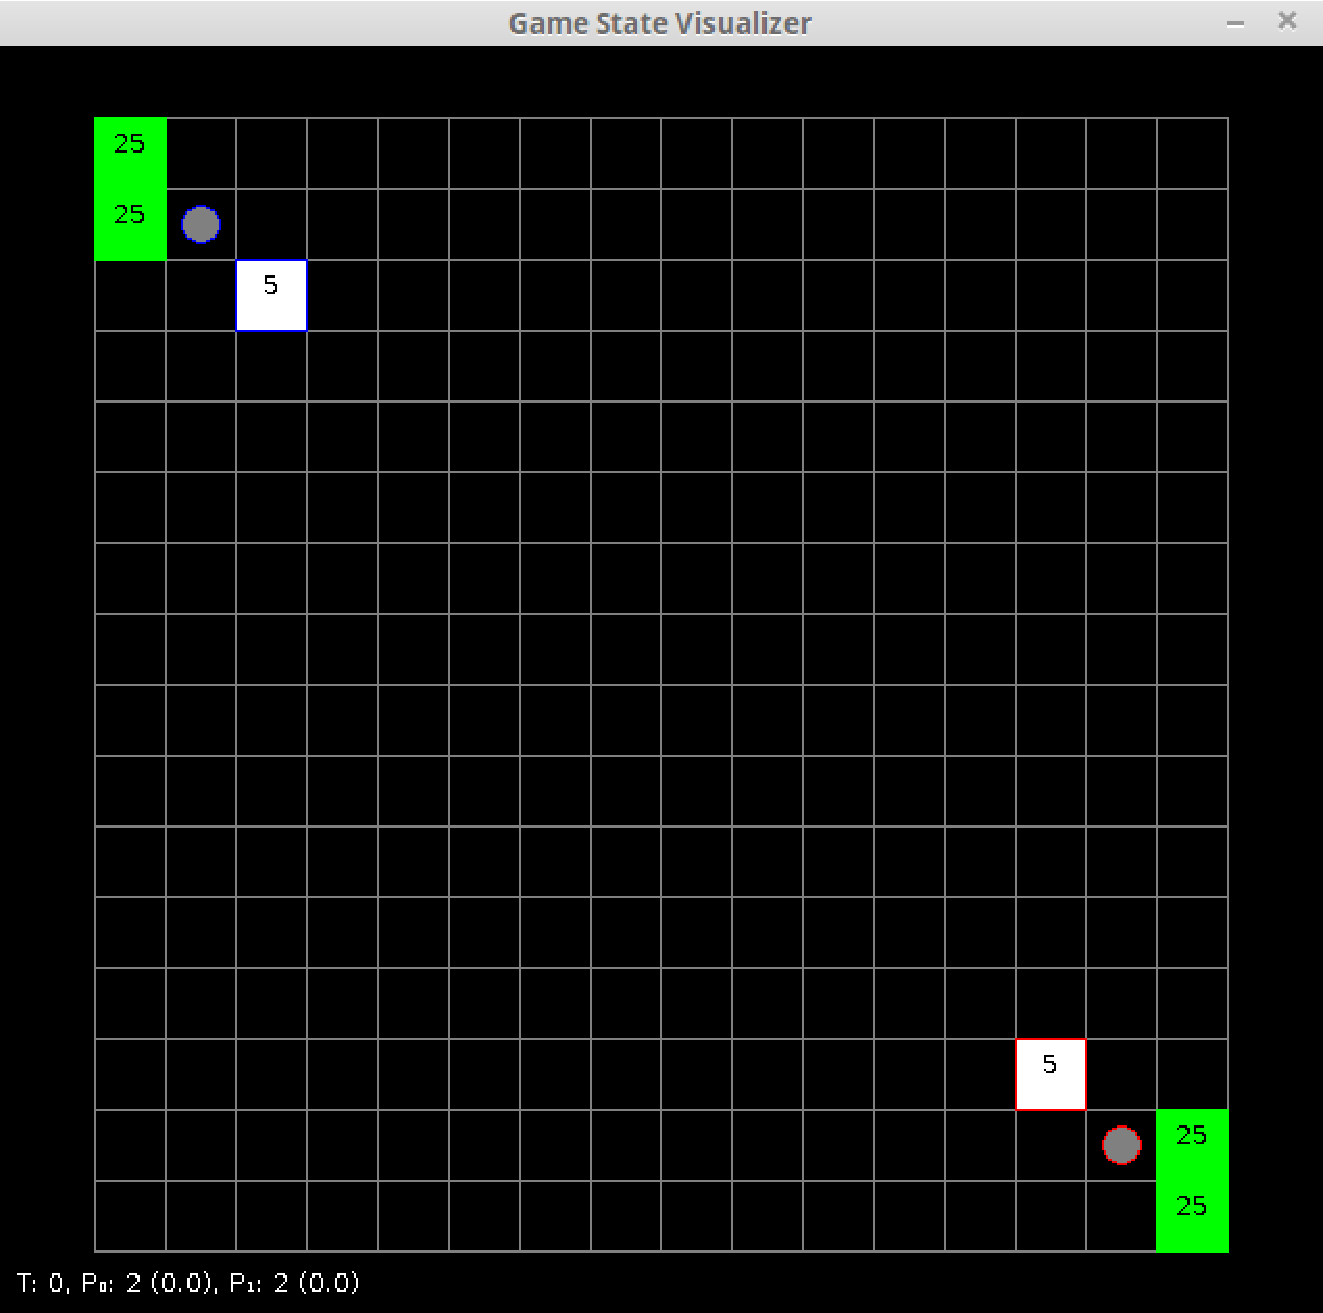
\includegraphics[width=.6\textwidth]{fig/map16x16.pdf}
	\caption{Diagrama de sequência}
	\label{fig:mapa16x16}
\end{figure}


explica a tabela


\begin{table}[]
	\centering
	\caption{Porcentagem de vitórias no mapa 1.}
	\label{tab:mapa1}
	\begin{tabular}{|c|cc|cc|}
		\hline
		\textbf{}           & \multicolumn{2}{c|}{\textbf{Estratégia 1}}  & \multicolumn{2}{c|}{\textbf{Estratégia 2}}  \\ \hline
		\textbf{Adversário} & \textbf{Lado Azul} & \textbf{Lado Vermelho} & \textbf{Lado Azul} & \textbf{Lado Vermelho} \\ \hline
		RandomIA            & 100\%              & 100\%                  & 100\%              & 100\%                  \\ \hline
		RandomBiasedIA      & 80\%               & 100\%                  & 100\%              & 100\%                  \\ \hline
		RangedRush          & 0\%                & 100\%                  & 100\%              & 100\%                  \\ \hline
		HeavyRush           & 0\%                & 100\%                  & 0\%                & 100\%                  \\ \hline
		LightRush           & 0\%                & 100\%                  & 0\%                & 100\%                  \\ \hline
		WorkerRush          & 0\%                & 0\%                    & 0\%                & 0\%                    \\ \hline
		MonteCarlo          & 60\%               & 80\%                   & 100\%              & 100\%                  \\ \hline
		Minimax             & 100\%              & 100\%                  & 100\%              & 100\%                  \\ \hline
		Portfolio           & 0\%                & 0\%                    & 0\%                & 0\%                    \\ \hline
	\end{tabular}
\end{table}

conclui alguma coisa

\section{Mapa 2}

\section{Mapa 3}

\section{Tamanho de cada IA}



\section{tempo de geração das ações do algoritmo}

Mostrar o tempo de gerar as ações que é alto no inicio e baixo no final
colocar gráficos aqui 


tempo para gerar as ações
da pra fazer uma tabela aqui com o tempo de cada técnica



\begin{itemize}
	\item BenchMark
	\item explicação dos resultados
	\item porcentagem de vitorias
	\item tempo de gerar cada ação
	\item tamanho de cada IA	
\end{itemize}


%!TEX root = volumeFinal.tex 

\chapter{\label{concl}Conclusões}

%----------------------------------------------------------------
% Após \appendix, se iniciam os capítulos de Apêndice, com
% numeração alfabética.
%----------------------------------------------------------------
\appendix
\include{estrategia1}
%!TEX root = volumeFinal.tex 

\chapter{\label{ap:estra2}Domínio HTN da estratégia 2}

\section{Domínio}


\lstset{style=codeStyle}
\begin{lstlisting}[language=lisp]
(defdomain ahtn-estrategia2
	(
		(:operator (!build-base ?worker ?recursoBase)
			((worker ?worker) (have ?recursoBase))
			((have ?recursoBase))
			((base ?base))
		)
		
		(:operator (!train-worker ?base ?recursoworker)
			((base ?base) (have ?recursoworker))
			((have ?recursoworker))
			((worker ?worker))
		)
		
		(:operator (!build-barrack ?worker ?recursoQuartel)
			((worker ?worker) (have ?recursoQuartel))
			((have ?recursoQuartel))
			((quartel ?quartel))
		)
		
		(:operator (!train-ranged ?quartel ?recursoRanged)
			((quartel ?quartel) (have ?recursoRanged))
			((have ?recursoRanged))
			((ranged ?ranged))
		)
		
		(:operator (!get-resource ?worker ?base ?recurso)
			((worker ?worker) (base ?base))
			()
			((have ?recurso))
		)
		
		(:operator (!attack-ranged ?ranged)
			((ranged ?ranged))
			()
			()
		)
		
		(:operator (!train-attack-ranged ?ranged)
			((ranged ?ranged) (quartel ?quartel) (have ?recursoRanged))
			((have ?recursoRanged))
			((ranged ?ranged))
		)
		
		(:method (construir-base ?base)
			((not (base ?base)) (recurso ?base ?recursoBase) (have ?recursoBase) (worker ?worker))
			((!build-base ?worker ?recursoBase))
		)
		
		(:method (treinar-worker ?worker)
			((not (worker ?worker)) (recurso ?worker ?recursoWorker) (have ?recursoWorker) (base ?base))
			((!train-worker ?base ?recursoWorker))
		)
		
		(:method (construir-quartel ?quartel)
			((not (quartel ?quartel)) (recurso ?quartel ?recursoQuartel) (have ?recursoQuartel) (worker ?worker)) 
			((!build-barrack ?worker ?recursoQuartel))
			
			((not (quartel ?quartel)) (recurso ?quartel ?recursoQuartel) (not (have ?recursoQuartel)) (worker ?worker) (base ?base))
			((!get-resource ?worker ?base ?recursoQuartel) (construir-quartel ?quartel))
			
			((not (quartel ?quartel)) (not (worker ?worker)) (base ?base))
			((treinar-worker ?worker) (construir-quartel ?quartel))
		
			((not (quartel ?quartel)) (not (base ?base)) (worker ?worker))
			((construir-base ?base) (construir-quartel ?quartel))
		)
		
		(:method (treinar-ranged ?ranged)
			((not (quartel ?quartel)))	
			((construir-quartel ?quartel) (treinar-ranged ?ranged))
			
			((quartel ?quartel) (recurso ?ranged ?recursoRanged) (not (have ?recursoRanged)) (worker ?worker) (base ?base))
			((!get-resource ?worker ?base ?recursoRanged) (treinar-ranged ?ranged))
			
			((quartel ?quartel) (recurso ?ranged ?recursoRanged))
			((!train-ranged ?quartel ?recursoRanged))
		)
		
		(:method (ataque-ranged ?ranged)
			((not (ranged ?ranged)))
			((treinar-ranged ?ranged) (ataque-ranged ?ranged))
			
			((ranged ?ranged) (quartel ?quartel) (recurso ?ranged ?recursoRanged) (have ?recursoRanged))
			((!train-attack-ranged ?ranged))
			
			((ranged ?ranged) (recurso ?ranged ?recursoRanged) (not (have ?recursoRanged)))
			((!attack-ranged ?ranged) (treinar-ranged ?ranged))
		)        
	)
)


\end{lstlisting}


%----------------------------------------------------------------
% Aqui vai a bibliografia. Existem 3 estilos de citação: use
% 'tcc-alpha' para citações do tipo [Abc+] ou [XYZ] (em ordem
% alfabética na bibliografia), 'tcc-num' para citações
% numéricas do tipo [1], [20], etc., em ordem de referência e
% 'tcc-alpha-full' para citações estilo 'alpha' mas com nomes completos.
%----------------------------------------------------------------
%\bibliographystyle{tcc-alpha-full}
\bibliographystyle{tcc-num}
\bibliography{referencias}



%----------------------------------------------------------------
% Aqui vão os "capítulos" de anexos. Cada anexo deve
% ser considerado um capítulo.
%----------------------------------------------------------------
%\anexos
%\chapter{Meu primeiro anexo}
%\chapter{My second attachment}

% E aqui (para a felicidade de todos) termina o documento.
\end{document}
